\documentclass{article}

\usepackage{fancyhdr}
\usepackage{extramarks}
\usepackage{amsmath}
\usepackage{amsthm}
\usepackage{amsfonts}
\usepackage{tikz}
\usepackage[plain]{algorithm}
\usepackage{algpseudocode}
\usepackage{enumerate}

\usetikzlibrary{automata,positioning}

%
% Basic Document Settings
%

\topmargin=-0.45in
\evensidemargin=0in
\oddsidemargin=0in
\textwidth=6.5in
\textheight=9.0in
\headsep=0.25in

\linespread{1.1}

\pagestyle{fancy}
\lhead{\hmwkAuthorName}
\chead{\hmwkClass\ (\hmwkClassInstructor\ \hmwkClassTime): \hmwkTitle}
\rhead{\firstxmark}
\lfoot{\lastxmark}
\cfoot{\thepage}

\renewcommand\headrulewidth{0.4pt}
\renewcommand\footrulewidth{0.4pt}

\setlength\parindent{0pt}

%
% Create Problem Sections
%

\newcommand{\enterProblemHeader}[1]{
    \nobreak\extramarks{}{Problem \arabic{#1} continued on next page\ldots}\nobreak{}
    \nobreak\extramarks{Problem \arabic{#1} (continued)}{Problem \arabic{#1} continued on next page\ldots}\nobreak{}
}

\newcommand{\exitProblemHeader}[1]{
    \nobreak\extramarks{Problem \arabic{#1} (continued)}{Problem \arabic{#1} continued on next page\ldots}\nobreak{}
    \stepcounter{#1}
    \nobreak\extramarks{Problem \arabic{#1}}{}\nobreak{}
}

\setcounter{secnumdepth}{0}
\newcounter{partCounter}
\newcounter{homeworkProblemCounter}
\setcounter{homeworkProblemCounter}{1}
\nobreak\extramarks{Problem \arabic{homeworkProblemCounter}}{}\nobreak{}

%
% Homework Problem Environment
%
% This environment takes an optional argument. When given, it will adjust the
% problem counter. This is useful for when the problems given for your
% assignment aren't sequential. See the last 3 problems of this template for an
% example.
%
\newenvironment{homeworkProblem}[1][-1]{
    \ifnum#1>0
        \setcounter{homeworkProblemCounter}{#1}
    \fi
    \section{Problem \arabic{homeworkProblemCounter}}
    \setcounter{partCounter}{1}
    \enterProblemHeader{homeworkProblemCounter}
}{
    \exitProblemHeader{homeworkProblemCounter}
}

%
% Homework Details
%   - Title
%   - Due date
%   - Class
%   - Section/Time
%   - Instructor
%   - Author
%

\newcommand{\hmwkTitle}{Tutorial Week 5}
\newcommand{\hmwkDueDate}{February 11, 2021}
\newcommand{\hmwkClass}{CZ4041}
\newcommand{\hmwkClassTime}{CS4}
\newcommand{\hmwkClassInstructor}{Assoc Prof Pan, Sinno Jialin}
\newcommand{\hmwkAuthorName}{\textbf{Pang Yu Shao}}
\newcommand{\hmwkAuthorID}{\textbf{U1721680D}}

%
% Title Page
%

\title{
    \vspace{2in}
    \textmd{\textbf{\hmwkClass:\ \hmwkTitle}}\\
    \normalsize\vspace{0.1in}\small{Due\ on\ \hmwkDueDate\ at 8:30am}\\
    \vspace{0.1in}\large{\textit{\hmwkClassInstructor\ - \hmwkClassTime}}
    \vspace{3in}\\
    \hmwkAuthorName\\
    \hmwkAuthorID
}

\date{11/02/2021}

\renewcommand{\part}[1]{\textbf{\large Part \Alph{partCounter}}\stepcounter{partCounter}\\}

%
% Various Helper Commands
%

% Useful for algorithms
\newcommand{\alg}[1]{\textsc{\bfseries \footnotesize #1}}

% For derivatives
\newcommand{\deriv}[1]{\frac{\mathrm{d}}{\mathrm{d}x} (#1)}

% For partial derivatives
\newcommand{\pderiv}[2]{\frac{\partial}{\partial #1} (#2)}

% Integral dx
\newcommand{\dx}{\mathrm{d}x}

% Alias for the Solution section header
\newcommand{\solution}{\textbf{\large Solution}}

% Probability commands: Expectation, Variance, Covariance, Bias
\newcommand{\E}{\mathrm{E}}
\newcommand{\Var}{\mathrm{Var}}
\newcommand{\Cov}{\mathrm{Cov}}
\newcommand{\Bias}{\mathrm{Bias}}

\begin{document}

\maketitle

\pagebreak

\begin{homeworkProblem}
    Consider the data set shown in Table 1 for a binary classification problem
    
    \begin{figure}[H]
        \begin{center}
        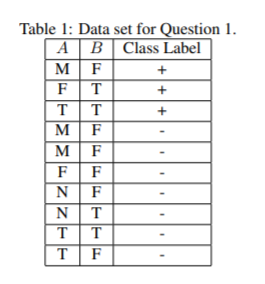
\includegraphics{resources/table1.PNG}
        \end{center}
    \end{figure}
    
    \begin{enumerate}
        \item Calculate the information gain when splitting on A and B (using multi-way
        split on A). Which feature would the decision tree induction algorithm choose?
        
        \item Calculate the gain ratio when splitting on A and B (using multi-way split on A).
        Which feature would the decision tree induction algorithm choose?
    \end{enumerate}
    

    \textbf{Solution}\\
    1.
    Information Gain: $\Delta_{info} = Entropy(parent\ node)-Entropy(children\ nodes)$
    \\
    \[
        \begin{split}
        E_p &= -(3/10)log_2(3/10) -(7/10)log_2(7/10)
        \\
            &= 0.88129
        \\\\
        E_A &= (3/10)(-(1/3)log_2(1/3) - (2/3)log_2(2/3)) + (2/10)(1) + (3/10)(-(1/3)log_2(1/3) - (2/3)log_2(2/3)) + (2/10)(0)
        \\
            &= 0.75097
        \\\\
        E_B &= (4/10)(1) + (6/10)(-(1/6)log_2(1/6) - (5/6)log_2(5/6))
        \\
            &= 0.79001
        \\\\
        \Delta_{info(A)} &= 0.88129 - 0.75097
        \\ 
        &= \mathbf{0.13032}
        \\
        \Delta_{info(B)} &= 0.88129 - 0.79001
        \\ 
        &= 0.09128
        \end{split}
    \]
    Therefore, the decision tree induction algorithm would choose to split on \textbf{A}.
    \newpage
    2.\\
    Gain Ratio: $\Delta_{InfoR} = \frac{\Delta_{info}}{SplitINFO}$\\\\
    Where  $SplitINFO = -\sum_{i=1}^{p}\frac{n_i}{n}log_2(\frac{n_i}{n})$
    \[
        \begin{split}
            SplitINFO_A &= -((3/10)log_2(3/10) + (3/10)log_2(3/10) + (2/10)log_2(2/10) + (2/10)log_2(2/10))
            \\
               &= -((6/10)log_2(3/10) + (4/10)log_2(2/10))
            \\
                &= 1.97095
            \\\\
            SplitINFO_B &= -((4/10)log_2(4/10) + (6/10)log_2(6/10))
            \\
                &= 0.97095
            \\\\
            \Delta_{infoR(A)} &= \Delta_{info(A)} / SplitINFO_A
            \\
            &=  0.13032 / 1.97095
            \\
            &= 0.06612
            \\
            \Delta_{infoR(B)} &= \Delta_{info(B)} /  SplitINFO_B
            \\
            &=  0.09128 / 0.97095
            \\
            &= \mathbf{0.09401}
        \end{split}
    \]
    Therefore, the decision tree induction algorithm would choose to split on \textbf{B}.


\end{homeworkProblem}

    



\end{document}